\documentclass[11pt]{amsart}
\usepackage{geometry}                % See geometry.pdf to learn the layout options. There are lots.
\geometry{letterpaper}                   % ... or a4paper or a5paper or ... 
%\geometry{landscape}                % Activate for for rotated page geometry
%\usepackage[parfill]{parskip}    % Activate to begin paragraphs with an empty line rather than an indent
\usepackage{graphicx}
\usepackage{amssymb}
\usepackage{epstopdf}
\usepackage{amsmath}
\usepackage[framed,numbered,autolinebreaks,useliterate]{mcode}
\DeclareGraphicsRule{.tif}{png}{.png}{`convert #1 `dirname #1`/`basename #1 .tif`.png}

\title{Scientific Computing Homework 2}
\author{Howard Jing and Sun Hyoung Sonya Kim}
%\date{}                                           % Activate to display a given date or no date

\begin{document}
\maketitle
\section*{Question 4.1}
In order to change Hermite polynomial basis of P$_{3}$ to Hermite basis of P$_{2}$, we can compose 3 linear transformations.

Let A be the linear transformation from Hermite polynomial basis of P$_{3}$ to power basis of P$_{3}$. According to page 73 of the textbook, that is:
 \[
A = \begin{bmatrix}
1 & 0 & -1& 0 \\
0 & 1 & 0 & -3 \\
0 & 0 & 1 & 0 \\
0 & 0 & 0 & 1
\end{bmatrix}^{-1}  = 
\begin{bmatrix}
1 & 0 & 1& 0 \\
0 & 1 & 0 & 3 \\
0 & 0 & 1 & 0 \\
0 & 0 & 0 & 1
\end{bmatrix}
\]

Let B be the linear transformation from power basis of P$_{3}$ to power basis of P$_{2}$. According to page 72 of the textbook, that is:
\[
B = \begin{bmatrix}
0 & 1 & 0& 0 \\
0 & 0 & 2 & 0 \\
0 & 0 & 0 & 3 
\end{bmatrix}
\]

Let C be the linear transformation from power basis of P$_{2}$ to Hermite polynomial basis of  P$_{2}$. According to page 73 of the textbook, that is:
\[
C = \begin{bmatrix}
1 & 0 & -1 \\
0 & 1 & 0 \\
0 & 0 & 1
\end{bmatrix}
\]

Then we can express the linear transformation from Hermite polynomial basis of P$_{3}$ to Hermite polynomial basis of  P$_{2}$ as compositions of linear transformations CBA:
\[
CBA = 
\begin{bmatrix}
1 & 0 & -1 \\
0 & 1 & 0 \\
0 & 0 & 1
\end{bmatrix} \cdot 
\begin{bmatrix}
0 & 1 & 0& 0 \\
0 & 0 & 2 & 0 \\
0 & 0 & 0 & 3 
\end{bmatrix}\cdot
\begin{bmatrix}
1 & 0 & 1& 0 \\
0 & 1 & 0 & 3 \\
0 & 0 & 1 & 0 \\
0 & 0 & 0 & 1
\end{bmatrix} =
\begin{bmatrix}
0 & 1 & 0& 0 \\
0 & 0 & 2 & 0 \\
0 & 0 & 0 & 3 
\end{bmatrix}
\]

Therefore the matrix that represents the differentiation operator that takes Hermite polynomial basis of P$_{3}$ to Hermite polynomial basis of P$_{2}$ is 
\[
\begin{bmatrix}
0 & 1 & 0& 0 \\
0 & 0 & 2 & 0 \\
0 & 0 & 0 & 3 
\end{bmatrix}
\]

\section*{Question 4.4}
\subsection*{a}
Since $V$ = $R^n$ and $M$ is an n$\times$n real matrix, for $u \in V$, $u^* = u^T$. Similarly, $M^* = M^T$. Because $u^*Mu$ is a $1\times1$ matrix,

\begin{align*}
u^*Mu &= (u^*Mu)^T\\
\iff u^TMu &= ((u^*M)(u))^T\\ &= u^T(u^*M)^T\\ &= u^TM^T(u^*)^T\\ &=u^TM^T{u^T}^T\\ &=u^TM^Tu\\
\implies u^*Mu &= u^*M^*u
\end{align*}
\\For $a \in R$, if $a= u^TMu$ then $a = u^TM^Tu$

\begin{align*}
a &= \frac{1}{2}a + \frac{1}{2}a\\
\implies a &= \frac{1}{2}(u^TMu) + \frac{1}{2}(u^TM^Tu)\\
&= u^T\frac{1}{2}Mu + u^T\frac{1}{2}M^Tu\\
& = u^T(\frac{1}{2}M + \frac{1}{2}M^T)u\\ 
&= u^*(\frac{1}{2}(M+M^*))u\\
\end{align*}

\subsection*{b}
For $a \in R$,
\begin{align*}
||au|| &= ((au)^TM(au))^\frac{1}{2}\\
&= (a^2 u^TMu)^\frac{1}{2}\\
&= (a^2)^\frac{1}{2}(u^TMu)^\frac{1}{2}\\
&= |a|||u||
\end{align*}
So $||.||$ is homogeneous.

\subsection*{c}
Given: $u^TMu > 0$ when $u\neq 0$.
\\We know that,
\[
||u|| = (u^TMu)^\frac{1}{2}
\]
\\For $u \neq 0$, 

\[u^TMu > 0 \implies (u^TMu)^\frac{1}{2} > 0\]
\\For $u = 0, $

\begin{align*}u = 0 &\implies Mu = 0\\ &\implies u^TMu = 0\\ &\implies (u^TMu)^\frac{1}{2} = 0\end{align*}
\\This means that $||u|| = 0$ if and only if $u = 0$ and is positive for all other $u$. Moreover, 
\[
||u|| \ge 0 \forall u
\]

\subsection*{d}
Lemma: For $u$, $v \in V$, and $M$, an $n \times n$ symmetric real matrix,
\[
u^TMv = v^TMu
\]
Proof: Note that $u^TMv = (u^TMv)^T$ because $u^TMv$ is a $1\times1$ matrix.
\begin{align*}
u^TMv &= (u^TMv)^T\\
&= ((u^TM)v)^T\\
&= v^T(u^TM)^T\\
&= v^TM^T{u^T}^T\\
&= v^TMu
\end{align*}

We know that $\phi (t) = (u+tv)^*M(u+tv) $ is a quadratic function of $t$ that is non-negative for all $t$ if $M$ is positive definite. This implies that,

\begin{align*}
0 \le \phi (t) &= (u+tv)^*M(u+tv)\\
&= u^TMu + u^TMtv + tv^TMu + tv^TMtv\\ 
&= u^TMu + tu^TMv + tu^TMu + t^2v^TMv\\
&= u^TMu + 2tu^TMv + t^2v^TMv \text{ (from Lemma)}\\
\end{align*}

We would like to find the minimum value of $\phi (t)$, but because $M$ is positive definite and $\phi (t)$ is quadratic, this simply means taking the derivative of $\phi (t)$ with respect to t and setting it equal to 0:

\begin{align*}
\phi (t) &= (v^TMv)t^2 + 2(u^TMv)t + u^TMu\\
\phi '(t) &= 2v^TMvT + 2u^TMv = 0\\
t &= \frac{-u^TMv}{v^TMv}
\end{align*}

Plug this value of t into the previous equation to get:
\begin{align*}
0 \le \phi (t) &= (v^TMv)(\frac{-u^TMv}{v^TMv})^2 + 2u^TMv(\frac{-u^TMv}{v^TMv}) + u^TMu\\
&= \frac{(-u^TMv)^2}{v^TMv} - \frac{2(u^TMv)^2}{v^TMv} + u^TMu\\
&= \frac{-(u^TMv)^2}{v^TMv} + u^TMu\\
\implies (u^TMv)^2 &\le (u^TMu)(v^TMv)\\
\implies (u^TMv)^2 &\le ||u||^2||v||^2\\
\implies |u^TMv| &\le ||u||||v|| \text{ (since $a^TMa \ge 0$ $\forall a$)}
\end{align*}
Which is the Cauchy Schwarz inequality.

\subsection*{e}
By applying the Cauchy Schwarz inequality, we know that
\[
||u||^2 + 2|u^TMv| + ||v||^2 \le ||u||^2 + 2||u||||v||+ ||v||^2
\]
However, note that
\begin{align*}
||u+v||^2 &= (u+v)^TM(u+v)\\
&= u^TMu + u^TMv + v^TMu + v^TMv\\
&= ||u||^2 + 2u^TMv + ||v||^2 \text{ (from Lemma)}\\
&= ||u||^2 + 2|u^TMv| + ||v||^2 \text{ (since $a^TMa \ge 0$ $\forall$ $a$)}\\
\end{align*}
Which means that 
\[
 ||u||^2 + 2|u^TMv| + ||v||^2 = ||u + v||^2 \le ||u||^2 + 2||u||||v||+ ||v||^2
\]
Which is the triangle inequality.

\subsection*{f}
If $M=I$, then $Mu = u$. This means that
\begin{align*}
(u^TMu)^\frac{1}{2} &= (u^Tu)^{1}{2}\\
&= ({u_1}^2 + {u_2}^2 + ... + {u_n}^2)^\frac{1}{2}
\end{align*}
Which is the definition of the $l_2$ norm.
\newline
\newline

\section*{Question 4.8}
\[
||A^{-1}|| = \max_{x \ne 0}{\frac{||A^{-1}x||}{||x||}} = \frac{1}{\min_{x \ne 0}{\frac{||x||}{||A^{-1}x||}}}
\]
Let A$^{-1}$x = y $\implies$ AA$^{-1}$x = Ay $\implies$ x = Ay. 

\[
||A^{-1}|| = \frac{1}{\min_{y \ne 0}{\frac{||Ay||}{||y||}}} =  \max_{y \ne 0}{\frac{||y||}{||Ay||}}
\]
\newline

\section*{Question 4.11}
\subsection*{a}

A must be a tridiagonal matrix of the form below in order for equation (4.45) to be set up properly.
\[
A = \begin{bmatrix}
-2 & 1 & 0 & \cdots & & 0 \\
1 & -2 & 1 &  &  & \vdots \\
0 & 1 & -2 & 1 &    \\
\vdots &  & 1 & -2 & \ddots  & 0\\
\vdots &  & & \ddots & \ddots & 1  \\
0 & \cdots & & 0 & 1 & -2
\end{bmatrix}
\]
\newline

In order to check that A has n-1 distinct eigenvectors having the form r$_{kj}$ = sin(k$\pi$x$_{j}$), find that A has n-1 distinct eigenvalues, which in turn implies that there are n-1 distinct eigenvectors. 

Eigenvectors have to satisfy the equation (Ar$_{k}$)$_{j}$ = $\lambda_{k}$r$_{kj}$
\[
\frac{1}{2(\Delta x)^2}[\sin(k\pi x_{j-1}) - 2\sin(k\pi x_{j}) + sin(k\pi x_{j+1})] = \lambda_{k}\sin(k\pi x_{j})
\]

\begin{align*}
\lambda_{k} &= \frac{\sin(k\pi(x_{j} - \Delta x)) - 2\sin(k\pi x_{j}) + \sin(k\pi(x_{j}+\Delta x))}{2(\Delta x)^2\sin(k\pi x_{j})}\\
&= \frac{\sin(k\pi x_{j}-k \pi \Delta x)-2\sin(k\pi x_{j})+\sin(k\pi x_{j}+k \pi \Delta x)}{2(\Delta x)^2\sin(k\pi x_{j})}\\
&= \frac{\sin(k\pi x_{j})\cos(k\pi \Delta x)-2\sin(k\pi x_{j}) + \sin(k\pi x_{j})\cos(k\pi \Delta x)}{2(\Delta x)^2\sin(k\pi x_{j})}\\
&= \frac{2\sin(k\pi x_{j})\cos(k\pi \Delta x)-2\sin(k\pi x_{j})}{2(\Delta x)^2\sin(k\pi x_{j})}\\
&= \frac{\cos(k\pi \Delta x)-1}{(\Delta x)^2}
\end{align*}

Since k$\Delta$x  $\le$ 1, and the periodicity of cosine is 2$\pi$, all of the eigenvalues $\lambda$$_{k}$'s are distinct. Thus there are n-1 distinct eigenvectors.

\subsection*{b}
From question 4.8, we established that 
\[
||A^{-1}|| = \max_{u \ne 0}{\frac{||u||}{||Au||}}
\]

But for which eigenvector is the value of the norm maximum? If we set u = r$_{min}$,
\[
\frac{||u||}{||Au||} = \frac{||r_{min}||}{|\lambda_{min}| ||r_{min}||}
= \frac{1}{|\lambda_{min}|}
\]

Indeed if we set u equal the smallest eigenvector, the norm of the inverse of A is maximized. Since we know $\lambda$$_{k}$, taylor expand it.
\begin{align*}
\lambda_{k} &= \frac{\cos(k\pi \Delta x)-1}{(\Delta x)^2}\\
&= \frac{1}{(\Delta x)^2} [1- \frac{(k\pi \Delta x)^2}{2}+ \cdot \cdot \cdot -1]\\
&= -\frac{(k\pi \Delta x)^2}{2(\Delta x)^2}\\
&= -\frac{(k\pi)^2}{2}
\end{align*}
By inspection of the expression for $|$$\lambda$$_{k}$$|$, note that $|$$\lambda$$_{1}$$|$ is the smallest, $|$$\lambda$$_{n-1}$$|$ is the largest.
\[
||A^{-1}|| = \frac{1}{|\lambda_{1}|}= \frac{1}{|-\frac{(\pi)^2}{2}|}=\frac{2}{\pi^2}
\]
\[
||A|| = |\frac{-((n-1)\pi)^2}{2}| = |\frac{n^2 \pi^2+2n\pi^2-\pi^2}{2}|
\]
\[\kappa(A) = ||A^{-1}||\cdot||A|| = (\frac{2}{\pi^2}) |\frac{n^2 \pi^2+2n\pi^2-\pi^2}{2}| = n^{2}+2n-1
\]
Therefore $\kappa$(A) = O(n$^{2}$) as n $\to$ $\infty$. 
\newline
\newline
\subsection*{c}
We know that $R = A\tilde{U} - F$, where the $j$th component of $\tilde{U}$, $u(x_j)$, is the exact but unknown solution to our problem. So the $j$th component of our residual R, $r_j$, is simply
\begin{align*}
r_j &= \frac{1}{2} \frac{1}{\Delta x^2}(u(x_j+\Delta x) - 2u(x_j) + u(x_j-\Delta x)) - F_j\\
&=\frac{1}{2} \frac{1}{\Delta x^2}(u(x_j+\Delta x) - 2u(x_j) + u(x_j-\Delta x)) - \frac{1}{2}u''(x_j)j\text{ (because $F_j = \partial_x^2 u_j)$ }
\end{align*} 

By Taylor expanding $u(x_j+\Delta x)$ and $u(x_j-\Delta x)$, we will show that every element of R will be of $O(\Delta x^2)$, which in turn implies that $||R|| = O(\Delta x^2)$.

Taylor expanding yields the following equations:
\begin{equation}
u(x_j + \Delta x) = u(x_j) + (\Delta x)u'(x_j) + \frac{1}{2}(\Delta x)^2 u''(x_j) + \frac{1}{3!}(\Delta x)^3u^{(3)}(x_j) + \frac{1}{4!}(\Delta x)^4u^{(4)}(x_j)+...
\end{equation}
\begin{equation}
\\u(x_j - \Delta x) = u(x_j) - (\Delta x)u'(x_j) + \frac{1}{2}(\Delta x)^2 u''(x_j) - \frac{1}{3!}(\Delta x)^3u^{(3)}(x_j) + \frac{1}{4!}(\Delta x)^4u^{(4)}(x_j)+...
\end{equation}

Adding $(1)$ and $(2)$ yields the following:

\begin{align*}
&u(x_j + \Delta x) + u(x_j - \Delta x) = 2u(x_j) + (\Delta x)^2 u''(x_j) + \frac{2}{4!}(\Delta x)^4u^{(4)}(x_j)+...\\
&\implies u(x_j + \Delta x) + u(x_j - \Delta x) - 2u(x_j) = (\Delta x)^2 u''(x_j) + \frac{2}{4!}(\Delta x)^4u^{(4)}(x_j)+...\\
&\implies \frac{1}{2}\frac{1}{\Delta x^2}[u(x_j + \Delta x) + u(x_j - \Delta x) - 2u(x_j)] = \frac{1}{2}u''(x_j) + \frac{1}{4!}(\Delta x)^4u^{(4)}(x_j)+...\\
\end{align*}

Finally, we have,
\[
r_j = \frac{1}{2}\frac{1}{\Delta x^2}[u(x_j + \Delta x) + u(x_j - \Delta x) - 2u(x_j)] - \frac{1}{2}u''(x_j) =  \frac{1}{4!}(\Delta x)^4u^{(4)}(x_j)+...\\
\]

Since every element in $R$ is of order $O(\Delta x^2)$, we conclude that $||R|| = O(\Delta x^2)$.

\subsection*{d}
R = A$\tilde{U}$ - F. Since F = AU $\implies$ R = A$\tilde{U}$ - AU = A($\tilde{U}$ - U)
\newline
Left multiply by A$^{-1}$ to get A$^{-1}$R = ($\tilde{U}$ - U)
\[
||\tilde{U} - U|| = || U - \tilde{U}|| = ||A^{-1}R|| \le ||A^{-1}||\cdot||R|| \le (\frac{2}{\pi^2})(O(\Delta x)^2)
\]
Thus $||$U - $\tilde{U}$$||$ = O($\Delta$x$^{2}$).

\subsection*{e}
We will use the method of undetermined coefficients to create a five point centered difference estimator for $\frac{\partial ^2 u}{\partial x}$. Let the ansatz be:
\[
u''(x) \simeq \frac{Au(x-2h) + Bu(x-h) + Cu(x) + Du(x+h) + Eu(x+2h)}{h^2}
\]
We will now choose the correct scalars $A$, $B$, $C$, $D$, and $E$.

Taylor expand $u(x-2h)$,$ u(x-h)$, $u(x+h)$, and $u(x+2h)$ to get the following:

\begin{align*}
u(x - 2h) &= u(x) - 2hu'(x) + \frac{2^2h^2}{2} u''(x) - \frac{2^3h^3}{3!}u^{(3)}(x) + \frac{2^4h^4}{4!}u^{(4)}(x)-\frac{2^5h^5}{5!}u^{(5)}(x)+...\\
u(x - h) &= u(x) - hu'(x) + \frac{h^2}{2} u''(x) - \frac{h^3}{3!}u^{(3)}(x) + \frac{h^4}{4!}u^{(4)}(x)-\frac{h^5}{5!}u^{(5)}(x)+...\\
u(x + 2h) &= u(x) + 2hu'(x) + \frac{2^2h^2}{2} u''(x) + \frac{2^3h^3}{3!}u^{(3)}(x) + \frac{2^4h^4}{4!}u^{(4)}(x)+\frac{2^5h^5}{5!}u^{(5)}(x)+...\\
u(x + h) &= u(x) + hu'(x) + \frac{h^2}{2} u''(x) + \frac{h^3}{3!}u^{(3)}(x) + \frac{h^4}{4!}u^{(4)}(x)+\frac{h^5}{5!}u^{(5)}(x)+...\\
\end{align*}

Plugging these values into our proposed approximation of $u''(x)$ then rearranging terms yields:
\begin{align*}
u''(x) &\simeq \frac{Au(x-2h) + Bu(x-h) + Cu(x) + Du(x+h) + Eu(x+2h)}{h^2}\\
&= A[u(x)-2hu'(x)+\frac{2^2h^2}{2}u^{(2)}(x)-\frac{2^3h^3}{6}u^{(3)}(x) + \frac{2^4h^4}{4!}u^{(4)}(x) - \frac{2^5h^5}{5!}u^{(5)}(x)+...]\\
&+B[u(x)-hu'(x)+\frac{h^2}{2}u^{(2)}(x)-\frac{h^3}{6}u^{(3)}(x) + \frac{h^4}{4!}u^{(4)}(x) - \frac{h^5}{5!}u^{(5)}(x)+...]\\
&+C[u(x)]\\
&+D[u(x)+hu'(x)+\frac{h^2}{2}u^{(2)}(x)+\frac{h^3}{6}u^{(3)}(x) + \frac{h^4}{4!}u^{(4)}(x) + \frac{h^5}{5!}u^{(5)}(x)+...]\\
&+E[u(x)+2hu'(x)+\frac{2^2h^2}{2}u^{(2)}(x)+\frac{2^3h^3}{6}u^{(3)}(x) + \frac{2^4h^4}{4!}u^{(4)}(x) + \frac{2^5h^5}{5!}u^{(5)}(x)]\\
\end{align*}
Which means that 
\begin{align*}
u''(x) &\simeq \frac{1}{h^2}(u(x)[A+B+C+D+E]  + hu'(x)[-2A -B + D + 2E]  \\ 
&+ h^2[2A + \frac{1}{2}B + \frac{1}{2}D + 2E]u''(x)  + h^3u^{(3)}(x)[\frac{-4}{3}A - \frac{1}{6}B + \frac{1}{6}D + \frac{4}{3}E]\\
&+ h^4u^{(4)}[\frac{2}{3}A + \frac{1}{24}B + \frac{1}{24}D + \frac{2}{3}E]+...)
\end{align*}
This implies the following conditions:
\begin{align*}
[A+B+C+D+E] &= 0\\
h[-2A -B + D + 2E]  &=0\\ 
h^2[2A + \frac{1}{2}B + \frac{1}{2}D + 2E] &=1\\
h^3[\frac{-4}{3}A - \frac{1}{6}B + \frac{1}{6}D + \frac{4}{3}E] &= 0\\
h^4[\frac{2}{3}A + \frac{1}{24}B + \frac{1}{24}D + \frac{2}{3}E] &= 0
\end{align*}
Solving the linear system of equations yields the values
\begin{align*}
A &= -\frac{1}{12}\\
B &= \frac{4}{3}\\
C &= -\frac{5}{2}\\
D &= \frac{4}{3}\\
E &= -\frac{1}{12}
\end{align*}
Our five point centered difference estimator is thus:
\begin{align*}
u''(x) & \simeq \frac{-\frac{1}{12}u(x-2h) +  \frac{4}{3}u(x-h) + -\frac{5}{2}u(x) + \frac{4}{3}u(x+h) + -\frac{1}{12}u(x+2h)}{h^2}\\
& = \frac{-u(x-2h) +  16u(x-h) -30u(x) + 16u(x+h) -u(x+2h)}{12h^2}
\end{align*}
Which is $O(n^4)$ accurate because the largest uncancelled error term will be $O(h^6)$, which when divided by $h^2$ will reduce to $O(h)^4$.

One solution for handling the case for j = 1 and j = n-1 is using 5-point uncentered difference that is biased to one side. So for example, for j=1, we would use the boundary value that is given u(0)=0 to its left and take 3 points to its right to account for j = -1. For j=n-1, we would take 3 points to its left, and use the right boundary value, u(n) = 0. 

If we were to keep using the 5-point centered difference method for the boundary cases, it would be fine to use U$_{0}$ = u(0) = 0. Since this is a given data, it will be acceptable to use for any function u(x).

\subsection*{f}
Matlab code  for solving AU=F

\begin{lstlisting}
function [normError] = boundaryValue(n)
    % takes step size as input (ie 0.01), outputs the norm of the error
    % set up our parameters

    step = 1/n;

    % set up our x and f(x)
    x = zeros(1,n-1);
    fx = zeros(1, n-1);
    U = zeros(1, n-1);

    x = [step:step:1 - step];
    fx = sin(pi*x);
    U = -sin(pi*x)/(2*(pi^2));

    % create the tridiagonal matrix A
    mainDiag = zeros(1, n-1);
    subDiag = zeros(1, n-2);
    A = zeros(n-1,n-1);

    mainDiag = -2*ones(1,(n-1));
    subDiag = ones(1,(n-2));

    A = diag(mainDiag, 0);
    A = A + diag(subDiag, 1);
    A = A + diag(subDiag, -1);
    A = 0.5 * (1/(step^2)) * A;
    
    % AU = fx, so solve for U
    appxU = zeros(n-1,1);
    appxU = A\fx';

    errors = abs(U' - appxU);
    errors = errors';
    
    normerr = 0;
    for i=1:(n-1)
        normerr = errors(i)^2;
    end
    normerr = sqrt(normerr);
    normError = normerr/(n-1);
end

function hw2_prob11
    n = [10:900:10000];
    steps = 1./n;
    errors = zeros(1, length(steps));
    errors = arrayfun(@boundaryValue, n);

    slopecheck = (steps).^2;
    
    figure
    loglog(steps, errors);
    title('Convergence Study of Second Order Method')
    xlabel('\Delta x')
    ylabel('Error(\Delta x)')
    hold on
    loglog(steps, slopecheck, 'r');
    legend('Error','Slope check with m = 2')
    hold off
end
\end{lstlisting}

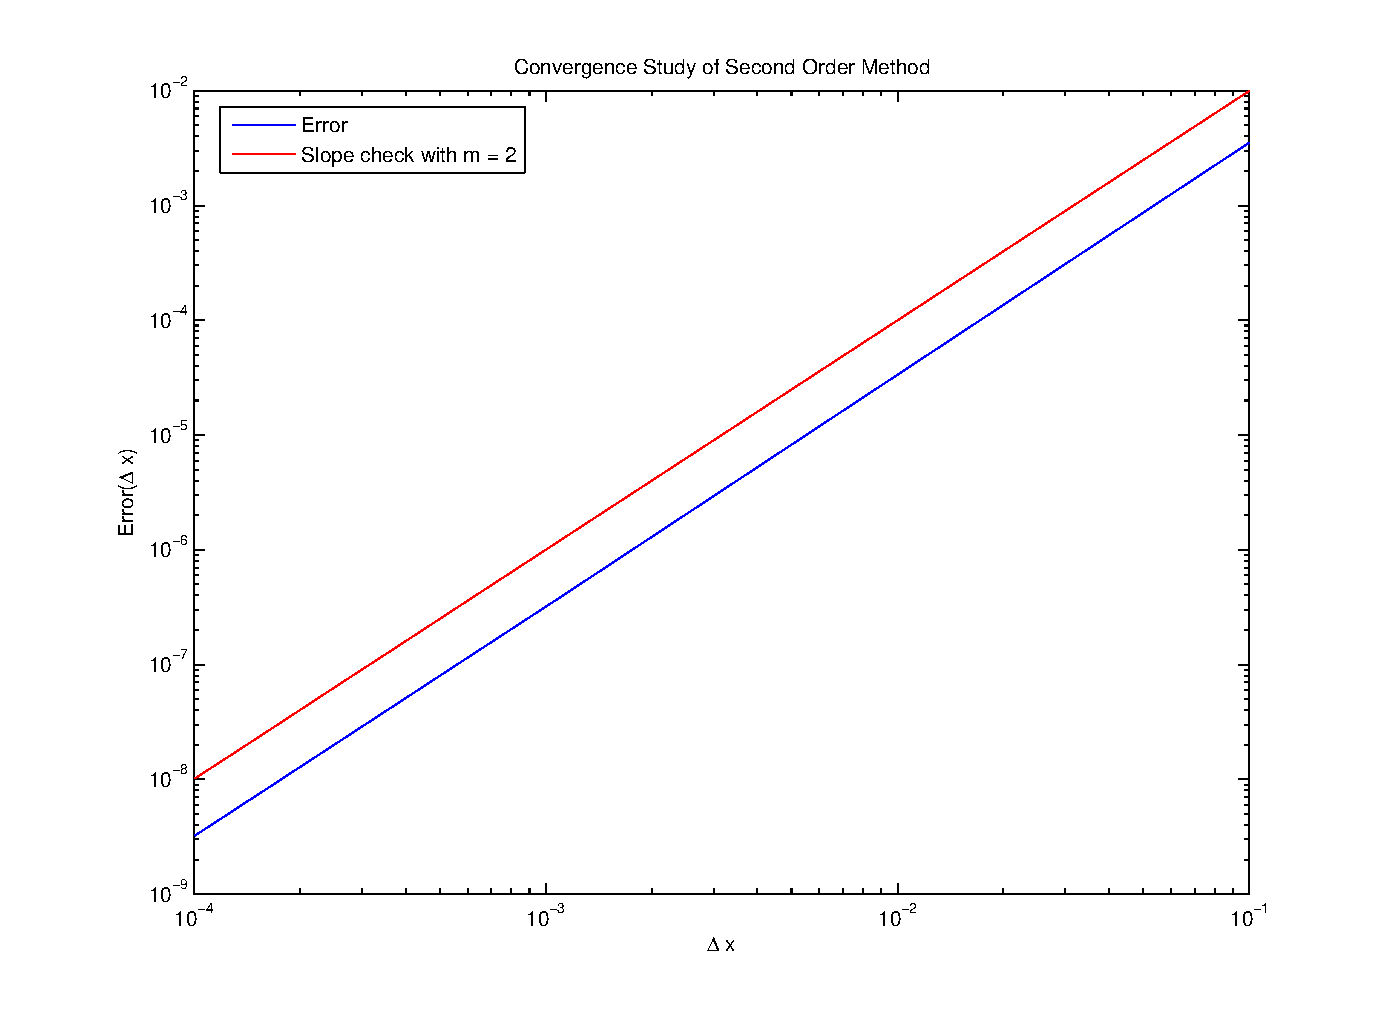
\includegraphics[height=4.5in]{11fdiagram.eps}

In above graph, the error is parallel to the test line that has a slope of 2. Therefore we can conclude that the results are indeed second order accurate. 

\subsection*{g}
Modifying the previous code to create a pentadiagonal Matrix A with coefficients as describe above for fourth order approximation.

\begin{lstlisting}
function [normError] = boundaryValue(n)
    % takes step size as input (ie 0.01), outputs the norm of the error
    % set up our parameters

    step = 1/n;

    % set up our x and f(x)
    x = zeros(1,n-1);
    fx = zeros(1, n-1);
    U = zeros(1, n-1);

    x = [step:step:1 - step];
    fx = sin(pi*x);
    U = -sin(pi*x)/(2*pi^2);

    % create the tridiagonal matrix A
    mainDiag = zeros(1, n-1);
    subDiag = zeros(1, n-2);
    A = zeros(n-1,n-1);

    mainDiag = (-5/2)*ones(1,(n-1));
    subDiag = (4/3)*ones(1,(n-2));
    subDiag2 = (-1/12)*ones(1,(n-3));
    

    A = diag(mainDiag, 0);
    A = A + diag(subDiag, 1);
    A = A + diag(subDiag, -1);
    A = A + diag(subDiag2, 2);
    A = A + diag(subDiag2, -2);
    A = (1/(step^2)) * A;

    %cond(A)
    % AU = fx, so solve for U
    appxU = zeros(n-1,1);
    appxU = A\fx';

    errors = abs(U' - appxU);
    errors = errors';
    
    normerr = 0;
    for i=1:(n-1)
        normerr = errors(i)^2 + normerr;
    end
    normerr = sqrt(normerr);
    %normError = norm(errors, 2)/(n-1);
    normError = normerr/(n-1);
end
\end{lstlisting}

Convergence study for fourth order method indicates that when f(x) = sin(x), the results are fourth order. However, when f(x) = max(0, .15-(x-.5)$^{2}$), the norm of the error is not O($\Delta$x$^{4}$). The difference in results relates to the fact that the second function is not analytic, which implies that the Taylor expansion of the function does not exist. 

\section*{Question 5.2}
A symmetric real $n \times n$ matrix $A$ is positive definite if and only if all its eigenvalues are positive.

If $A$ is positive definite, then $\forall x \in R^n$ and $x \ne 0$ we know that $x^TAx > 0$. Also, $\forall$ eigenvectors $y$ of $A$, $\exists$ $\lambda \in R$ such that $Ay = \lambda y$,

\begin{align*}
\implies y^TAy &> 0\\
\iff y^T\lambda y &> 0\\
\iff \lambda y^Ty &>0\\ 
\end{align*}

Because the dot product $y^Ty$ is always nonnegative, we conclude that for every eigenvalue $\lambda$ of $A$, $\lambda$ must be positive for the above inequality to hold.

To prove that if all of $A$'s eigenvalues are positive, note that if $A$ is symmetric, then $A$ can be decomposed into $A = R\Lambda R^T$, where $\Lambda$ is a diagonal matrix containing the eigenvalues of $A$. This means that $x^TAx = x^TR\Lambda R^Tx = y^T\Lambda y$ where $y = R^Tx$. Then if every diagonal entry of $\Lambda$ is positive implies that $y^T\Lambda y$ is positive definite, the proof is finished.
If $y=0$, then $y^T\Lambda y = 0$. Otherwise note that,

\begin{align*}
y^T\Lambda y = \sum_{k=1}^{n} \lambda _k {y_k}^2 \implies \sum_{k=1}^{n} \lambda _k {y_k}^2 & > 0 
\end{align*}
because $\lambda _k, {y_k}^2$ are both greater than 0. This implies that $y^T \Lambda y > 0$ for $y \ne 0$ $\iff x^TAx > 0$ for $x \ne 0 $. So $A$ is positive definite. 

If $A$ is symmetric positive definite, then there are distinct linearly independent eigenvectors that form a basis. So the $x$ that when applied to $x^TAx$ that gives the smallest number would be the eigenvector that corresponds to $\lambda _{min}$, the smallest eigenvalue of $A$. This implies the following,

\begin{align*}
Ax &= \lambda x\\
x^TAx &= x^T\lambda x\\
&= \lambda x^Tx\\
&= \lambda ||x||^2\\
\end{align*}
Because we know that $\lambda _{min}$ must be positive, we conclude that $x^TAx > \lambda _min ||x||^2$ for all $x$.
\newline
\newline
\end{document}  

\pdflatex